In this section we connect three load generating VMs to two middlewares and three memchached servers. We only run write-only workloads and we want to figure out the effects of replicating data to the servers. The experimental setup is the same as in the previous section.  

\subsection{Full System}
The overview of the experiment parameters is given in the following table:
\begin{center}
	\scriptsize{
		\begin{tabular}{|l|c|}
			\hline Number of servers                & 3          \\ 
			\hline Number of client machines        & 3          \\ 
			\hline Instances of memtier per machine & 2          \\ 
			\hline Threads per memtier instance     & 1          \\
			\hline Virtual clients per thread       & \{1,4,8,16,24,32,48\}    \\ 
			\hline Workload                         & Write-only \\
			\hline Number of middlewares            & 2          \\
			\hline Worker threads per middleware    & \{8,16,32,64\}   \\
			\hline Repetitions                      & 3   \\ 
			\hline 
		\end{tabular}
	} 
\end{center}
% plots
The throughput and response time as a function of virtual clients for write-only workloads is shown in Figure \ref{full_write_tp} and in Figure \ref{full_write_rt}. 
\begin{figure}[H]
   \begin{minipage}{0.48\textwidth}
     \centering
     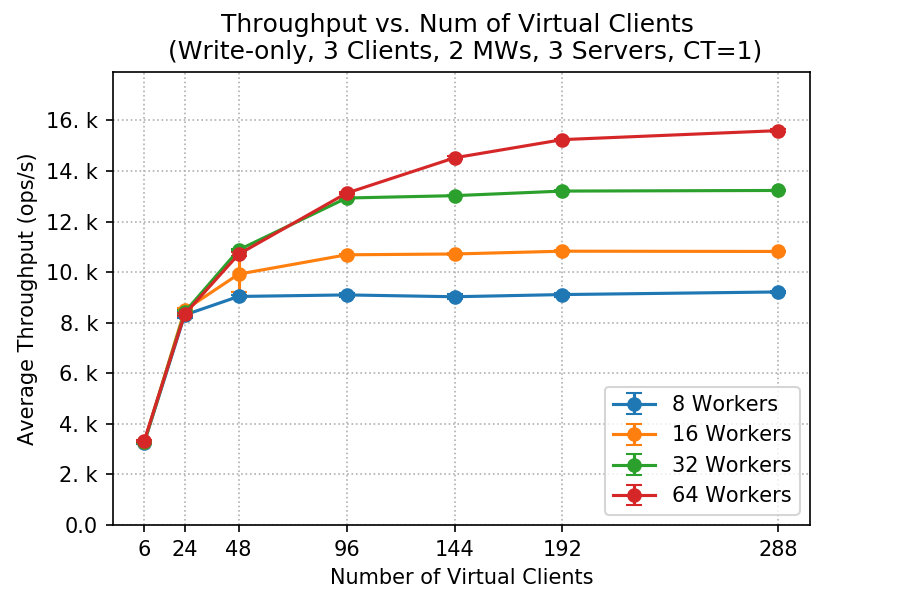
\includegraphics[width=1\linewidth]{figures/3_ThroughputForWrites/full_write_mw_tp_write_2018-11-09_13h02.png}
     \caption{Throughput of middlewares}\label{full_write_tp}
   \end{minipage}\hfill
   \begin{minipage}{0.48\textwidth}
     \centering
     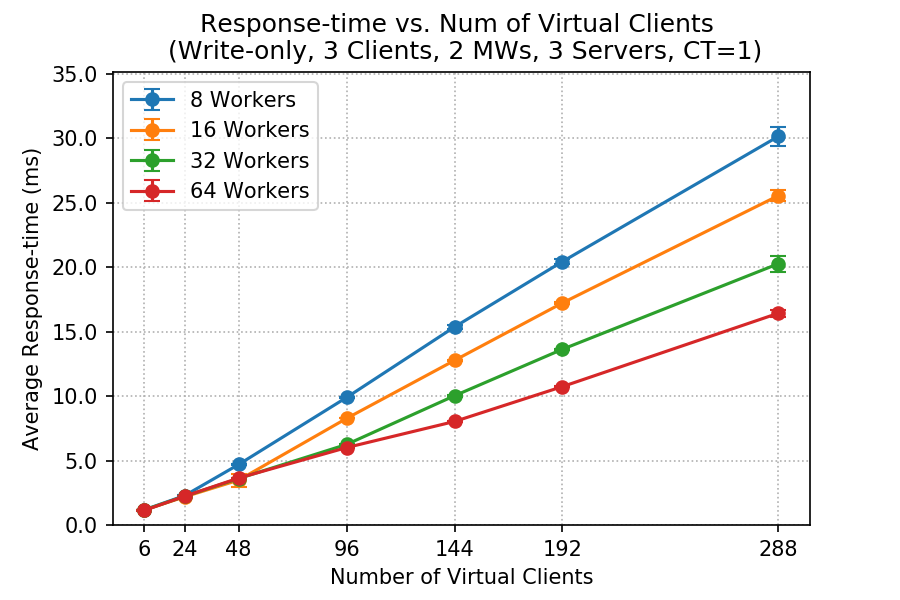
\includegraphics[width=1\linewidth]{figures/3_ThroughputForWrites/full_write_rt_write_2018-11-09_13h02.png}
     \caption{Response time of middlewares}\label{full_write_rt}
   \end{minipage}
\end{figure}

%% explanation
In Figure \ref{full_write_tp} and Figure \ref{full_write_rt} we can see that saturation for 8 workers is reached at 24 clients, for 16 workers at 48 clients, for 32 workers at 96 clients and for 64 workers at 192 clients because at those points throughput starts to flatten and we also see the response time increasing more significantly. 

First of all, we can compare the response time measured at the middleware with Section \ref{sec:baselineWithMWTwo} (write-only workload), where we have one instead of three servers. Comparing Figure \ref{two_mws_rt_write} and Figure \ref{full_write_rt} we see that the response time does slightly increase if we take three instead of one server, which makes sense because we have to additionally replicate the data in this experiment. A worker thread sends a Set request from the client to each server, one after the other, and then waits until all Set requests have been executed on all servers, which leads to a longer response time on the middleware. 

The bottleneck for all four worker configurations are the worker threads themselves. To see this we can first look at the average queue length (Figure \ref{queue_length_full_write}). We see that the queue length starts increasing significantly at the mentioned saturation points. We have queue congestion because the arrival rate into the queue is bigger than the combined service rate of the worker threads. 

\begin{figure}[H]
   \begin{minipage}{0.48\textwidth}
        \centering
	    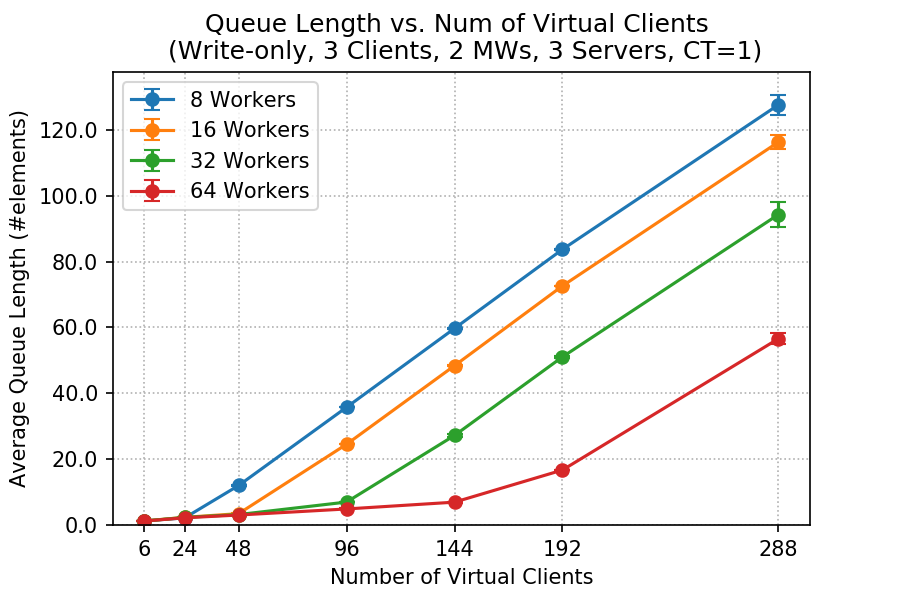
\includegraphics[scale=0.48]{figures/3_ThroughputForWrites/full_write_mw_queuelength_write_2018-11-09_13h02.png}
	    \caption{Average queue length.}
	    \label{queue_length_full_write}
   \end{minipage}\hfill
   \begin{minipage}{0.48\textwidth}
        \centering
	    \includegraphics[scale=0.48]{figures/3_ThroughputForWrites/dstat_mw_netsend_ratio_1:0_2018-11-09_13h02.png}
	    \caption{Outbound network activity of the middlewares.}
	    \label{outbound_mw_network_acitivity_full_write}
   \end{minipage}
\end{figure}
% look at outbound network bandwidth of middleware
We also checked the outbound network bandwidth at the middlewares because the middlewares have to send three times more data than in the one server case due to replication. Figure \ref{outbound_mw_network_acitivity_full_write} shows the outbound network activity of a middleware VM. We found out with \textit{iperf} that the maximum outbound bandwidth of a middleware VM is 100 MBps, which is almost reached for 64 workers. But since it is not reached at the saturation point, it is not the reason for saturation and thus not the bottleneck for the 64 workers case. 

We can support our bottleneck analysis by additionally looking at the response time of the middleware in more detail (Figure \ref{rt_breakdown_write_full_write}). We can also see that the queue time starts increasing at the saturation points.
The increase in waiting time for memcached (denoted as "Memcached RTT") for higher number of workers also makes sense because servers need to serve more workers simultaneously. 
\begin{figure}[H]
    \centering
	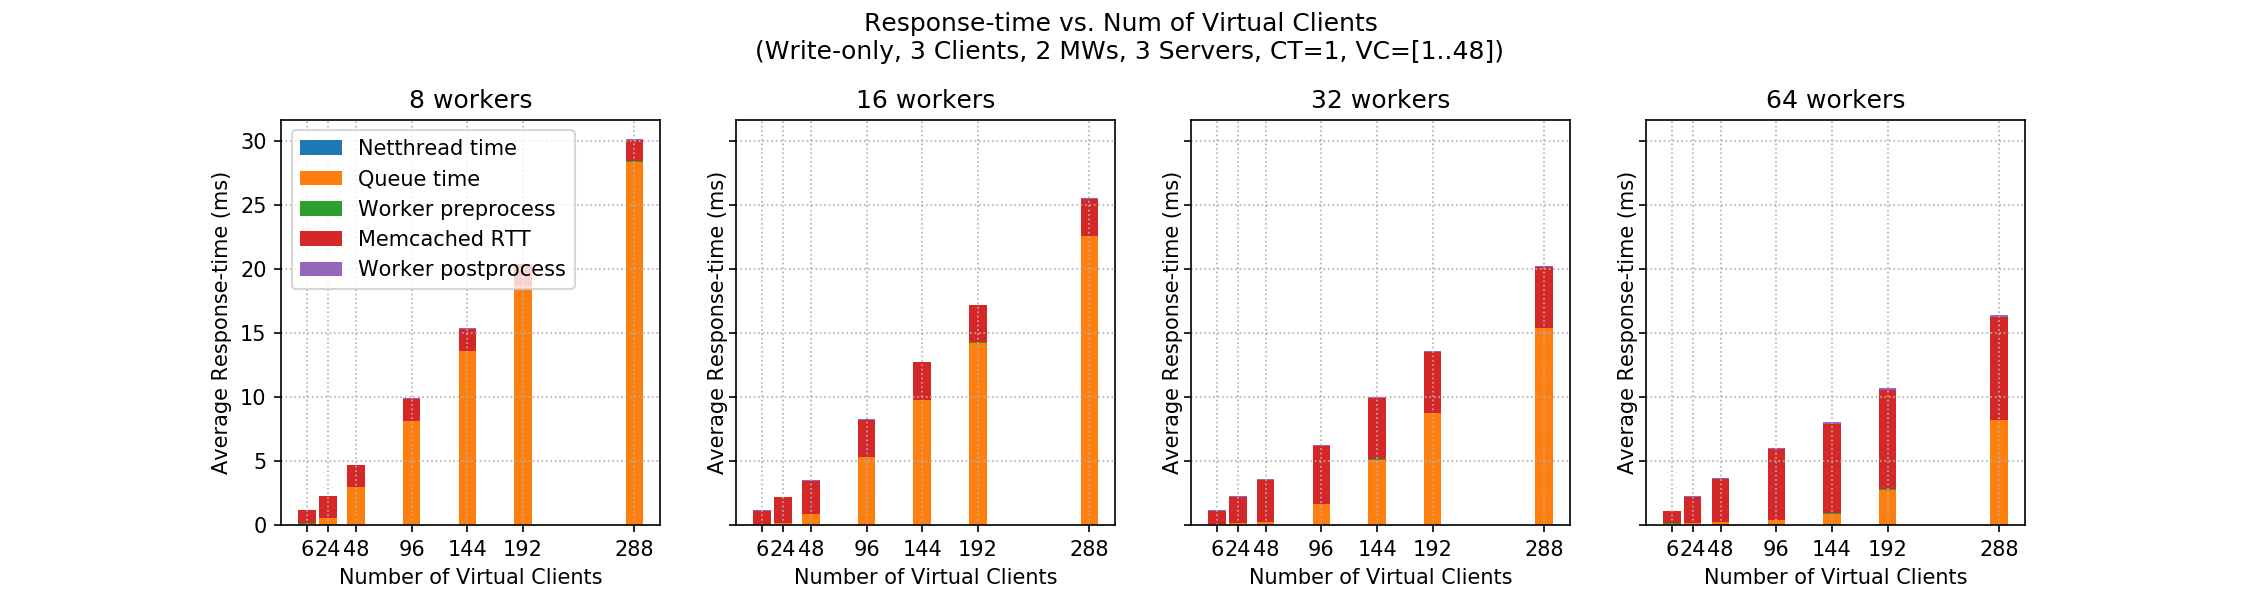
\includegraphics[scale=0.48,width=\linewidth]{figures/3_ThroughputForWrites/full_write_mw_rt_breakdown_write_2018-11-09_13h02.png}
	\caption{Response time breakdown.}
	\label{rt_breakdown_write_full_write}
\end{figure}

% analyze CPU utilization
%Our first guess is the CPU utilization of the servers because this is also the bottleneck for 64 worker threads in the one server case. Figure \ref{cpu_full_write} shows that this is not the case for three servers. We see that CPU utilization increases with more worker threads because the memcached threads have to maintain more connections in parallel and serve more requests but it is not the bottleneck.
%\begin{figure}[H]
%    \centering
%	\includegraphics[scale=0.48]{figures/3_ThroughputForWrites/dstat_server_cpu_ratio_1:0_2018-11-09_13h02.png}
%	\caption{CPU utilization of server VMs.}
%	\label{cpu_full_write}
%\end{figure}

% analyze mw bandwidth netsend
%Let us analyze the bottleneck for the \textbf{64 worker threads} setting. 
%Our guess is that the outbound network bandwidth at the middlewares is the bottleneck because the middlewares have to send %three times more data than in the one server case because of replication. Figure \ref{outbound_mw_network_acitivity_full_write} shows that this is indeed the case. We checked with \textit{iperf} that the maximum outbound bandwidth of a middleware VM is around 100 MBps which is reached in this case for the 64 worker setting.

\subsection{Summary}

\begin{center}
	{Maximum throughput for the full system}
	\begin{tabular}{|l|p{2.1cm}|p{2.1cm}|p{2.1cm}|p{2.1cm}|}
		\hline                                            & WT=8 & WT=16 & WT=32 & WT=64 \\ 
		\hline Throughput (Middleware)                    & 8'304 ops/s & 8'480 ops/s & 12'930 ops/s & 14'519 ops/s	       \\ 
		\hline Throughput (Derived from MW rt)            & 7'565 ops/s & 7'795 ops/s & 13'440 ops/s & 16'134 ops/s \\ 
		\hline Throughput (Client)                        &8'284 ops/s & 8'498 ops/s & 12'905 ops/s & 14'457 ops/s       \\ 
		\hline Average time in queue                      &0.54ms&0.14ms&1.59ms&0.8ms	 \\ 
		\hline Average length of queue                    &2.16 & 2.32 & 6.97 & 6.93 \\ 
		\hline Average time waiting for memcached         & 1.67ms  & 1.98ms & 4.51ms & 6.99ms	 \\ 
		\hline 
	\end{tabular}
\end{center}
% choice of configurations that give max throughput
The configurations that give maximal throughput are chosen such that a good trade-off between the throughput and latency is achieved. For 8 workers, 24 clients were chosen because going from 24 to 48 clients would increase response time by $84\%$, while only increasing throughput by $8.8\%$. For 16 workers, also 24 clients were chosen because going from 24 clients to 48 clients would increase response time by $55\%$, while only increasing throughput by $16\%$. For 32 workers, 96 clients were chosen because going from 96 to 144 clients would increase response time by $50\%$, while only increasing throughput by less than $1\%$. For 64 workers, 144 clients were chosen because going from 144 to 288 clients would increase response time by $28\%$, while only increasing throughput by $5\%$.

% interactive law
The throughput can be derived from the MW response time in two ways using the interactive law: Either we consider the round-trip time between the MWs and the clients as the waiting time Z or we adjust the number of requests N by subtracting the average number of requests that are between the clients and the middlewares. We choose the first approach and average the ping times between the clients and the middlewares to get an average round-trip time of 0.8915ms. 
% explain
For 64 workers the throughput derived from the middleware response time is significantly overestimated. This is because the difference between the response time measured at the client and at the middleware is larger than the network latency between them and thus the think time Z is chosen too small. This difference includes the time a request waits in front of the net-thread. The more worker threads there are, the more threads compete for the same resource, which slows down the net-thread.

% Draw conclusions on the state of your system for a variable number of worker threads.
The highest throughput is reached with 64 worker threads. This is because the workers are the bottleneck in this setup and in general increasing the resource at a bottleneck increases the throughput of a system. Thus we achieve highest throughput with the highest number of workers.
With 64 worker threads and high enough load, the maximum outbound network bandwidth of the middleware VMs is almost reached (Figure \ref{outbound_mw_network_acitivity_full_write}) which means that going beyond 64 workers would not significantly increase the throughput anymore in this setup. In order to reduce the network send activity of the middleware VMs such that one can increase the throughput even more, one would have to either increase the number of middlewares or decrease the replication factor of the key-value pairs.

